\documentclass[11pt,a4paper]{article}
\usepackage[margin=2.2cm,headheight=14pt]{geometry}
\usepackage[T1]{fontenc}
\usepackage{lmodern}
\usepackage{microtype}
\usepackage{booktabs}
\usepackage{graphicx}
\usepackage[table]{xcolor}
\usepackage{caption}
\usepackage{subcaption}
\usepackage{float}
\usepackage{needspace}
\usepackage{enumitem}
\usepackage{amsmath}
\usepackage{fancyhdr}
\usepackage{titlesec}
\usepackage[most]{tcolorbox}
\usepackage[hidelinks]{hyperref}

\definecolor{ink}{HTML}{1B2A41}
\definecolor{accent}{HTML}{0F7B8A}
\definecolor{soft}{HTML}{E8F3F5}
\definecolor{mute}{HTML}{6B7785}

\setlist{itemsep=1pt,topsep=2pt}
\captionsetup{font=small,labelfont={bf,color=ink}}
\graphicspath{{figures/}}
\newcommand{\code}[1]{\texttt{#1}}

\titleformat{\section}{\Large\bfseries\color{ink}}{\thesection}{0.6em}{}[{\color{accent}\titlerule[0.8pt]}]
\titleformat{\subsection}{\large\bfseries\color{ink}}{\thesubsection}{0.5em}{}
\titlespacing*{\section}{0pt}{14pt}{6pt}
\titlespacing*{\subsection}{0pt}{9pt}{3pt}
\renewcommand{\arraystretch}{1.08}

\pagestyle{fancy}
\fancyhf{}
\renewcommand{\headrulewidth}{0.3pt}
\fancyhead[L]{\small\color{mute}ML Final Project}
\fancyhead[R]{\small\color{mute}Traffic Prediction, Topic 4}
\fancyfoot[C]{\small\thepage}

\newtcolorbox{keybox}[1][]{colback=soft,colframe=accent,boxrule=0.6pt,arc=2pt,left=8pt,right=8pt,top=6pt,bottom=6pt,#1}

\begin{document}
\thispagestyle{empty}
% ---------------------------------------------------------------------------------------------- title block
\begin{center}
{\fontsize{24}{28}\selectfont\bfseries\color{ink} ML Final Project (Traffic Prediction)}
\end{center}
\vspace{-2pt}
{\color{accent}\rule{\linewidth}{1.2pt}}
\vspace{4pt}

\noindent
\begin{minipage}[b]{0.55\linewidth}
{\large\color{mute} Forecasting freeway flow 15 and 60 minutes ahead at 100 Bay Area sensors (LargeST, 2017--2019)}\\[6pt]
{\small Topic 4, Traffic Prediction\\
Code and README: \url{https://github.com/praneethem/Traffic-Prediction}}
\end{minipage}\hfill
\begin{minipage}[b]{0.40\linewidth}\raggedleft
\textbf{Praneeth Marudi} (IMT2023555)\\[2pt]
\textbf{Vinay Kusumanchi} (IMT2023608)\\[2pt]
\textbf{Shive S Bhat} (BT2024067)\\[2pt]
\textbf{Mitansh Shringi} (BT2024046)
\end{minipage}

\vspace{6pt}
{\color{accent}\rule{\linewidth}{0.5pt}}
\vspace{6pt}

\noindent\textbf{\color{accent}Summary.} We forecast the traffic flow (vehicles per 15 minutes) at 100 freeway sensors of the San Francisco Bay Area,
15 and 60 minutes ahead, from the public LargeST dataset. Nine models and three simple baselines are compared on identical rows.
Models are tuned on 2017--2018, frozen, and scored once on 2019. LightGBM is best: MAE 48.63 (15 min) and 61.15 (60 min),
26.7\% and 22.0\% better than the best baseline. XGBoost and CatBoost are practically tied with it. Recent flow, the calendar and
last week's pattern carry the forecasts; weather and PCA add nothing. The largest errors come from sudden changes, holidays and
data outages.

% ---------------------------------------------------------------------------------------------- 1
\section{Overview and task definition}
The task is to forecast the traffic flow at each of 100 freeway sensors at two horizons, \textbf{15 and 60 minutes ahead}.
Flow is the number of vehicles that crossed a loop detector in a 15-minute \emph{bin}; all errors are in vehicles per 15 minutes.
A forecast is made at an \emph{origin}: every reading of bins that have completed is known, nothing later.
Bins are labelled by their start time, so the latest known bin is the one before the origin. The 15-minute target is the next bin
(starting at the origin); the 60-minute target is the bin that ends 60 minutes after the origin. We train one model per horizon,
shared by all sensors.

The study compares Ridge regression, PCA followed by Ridge, a Decision Tree, a Random Forest and five boosting methods (AdaBoost,
Gradient Boosting, XGBoost, LightGBM, CatBoost) against three baselines, with six analyses (what the models rely on,
how robust they are, where they fail, and more) and a working web app. Figure~\ref{fig:flow} shows the pipeline.

\begin{figure}[H]\centering
\footnotesize
\begin{tabular}{@{}c@{\;}c@{\;}c@{\;}c@{\;}c@{\;}c@{}}
\fcolorbox{accent}{soft}{\parbox{0.118\linewidth}{\centering raw 5-min flow, 100 sensors}} $\to$ &
\fcolorbox{accent}{soft}{\parbox{0.118\linewidth}{\centering fault flags, 15-min bins, causal fill}} $\to$ &
\fcolorbox{accent}{soft}{\parbox{0.118\linewidth}{\centering scale target, 31 features}} $\to$ &
\fcolorbox{accent}{soft}{\parbox{0.118\linewidth}{\centering chronological split, purge}} $\to$ &
\fcolorbox{accent}{soft}{\parbox{0.118\linewidth}{\centering 9 models, tune on 2018}} $\to$ &
\fcolorbox{accent}{soft}{\parbox{0.118\linewidth}{\centering frozen test 2019, analyses, app}}
\end{tabular}
\caption{Pipeline from raw readings to the frozen 2019 test.}\label{fig:flow}
\end{figure}

\noindent\textbf{Where each requirement is covered.} EDA and preprocessing: Sections 3--4, split in Section 6. Benchmarking of PCA, Decision Tree, Random Forest and five boosting variants: Sections 7--8. Analyses A, B, C, D, E, F: Section 9. UI: Section 10. Leakage prevention: Section 5. Limitations and conclusions: Section 11.

% ---------------------------------------------------------------------------------------------- 2
\section{Dataset and source}
\textbf{Traffic.} LargeST \cite{largest} is a public benchmark built from Caltrans PeMS loop detectors \cite{pems}. We use its Greater
Bay Area part: 5-minute counts for 2017--2019 and sensor metadata (freeway, direction, county, lanes, coordinates). Licence CC BY-NC 4.0. An automated test confirms the 5-minute and 15-minute tables have unique timestamps in regular steps, with 365 full days in each year, so there are no missing or duplicated rows; every gap is a missing value.\\
\textbf{Sensors.} 100 sensors in four corridors of 25 consecutive sensors each: I-580 East, US-101 North, I-880 South and SR-24 West,
chosen for data quality (each has at least about 99\% usable readings in both 2017 and 2018). Within a corridor, the first 20 sensors
are \emph{warm} (used in training, tuning and test) and the last 5 are \emph{cold}: they appear only in 2019 test rows, so they show
whether a model works on a sensor it has never seen. Warm sensors never use cold sensors as neighbours.\\
\textbf{Weather.} Hourly precipitation, temperature and wind per corridor from the Open-Meteo historical API \cite{openmeteo}, which serves the
ERA5 reanalysis. It is area weather, not measured at the sensors.

% ---------------------------------------------------------------------------------------------- 3
\section{Exploratory data analysis}
EDA used 2017--2018 only (2019 is never opened). Each finding led to a decision:
\begin{itemize}
\item \textbf{Daily and weekly rhythm.} Weekdays show commute peaks, weekends one midday hump; weekend flow is about 0.86 of weekday
flow and holidays behave like weekends. $\Rightarrow$ calendar and same-time-last-week features (Figure~\ref{fig:eda}a).
\item \textbf{Neighbours move together.} After removing the typical pattern, adjacent sensors correlate about 0.50
(Figure~\ref{fig:eda}b). $\Rightarrow$ neighbour features.
\item \textbf{Missing data is rare but clumpy.} 0.29\% of readings are missing, but the median gap lasts 4 hours and 70\% of gaps exceed one hour.
$\Rightarrow$ fault flags and causal imputation; no interpolation, which would use the future.
\item \textbf{Faulty readings.} Long daytime zero runs, long runs of one repeated value, and impossible values. $\Rightarrow$ marked missing.
\item \textbf{Template sensors.} About 10\% of sensor-days only repeat the reading from 7 days earlier or later, and 8 sensors do so almost
every day. $\Rightarrow$ a ``clean rows'' view in the results (Sections~\ref{sec:prep} and \ref{sec:clean}).
\item \textbf{Weather has a small effect.} Rain lowers flow by about 2.8\% in a matched comparison. $\Rightarrow$ weather features, expected to add little.
\item \textbf{Changes between bins} are usually small (median 5\% of the sensor's level) but have a heavy tail (99th percentile 39\%), and
sensors differ hugely in size. $\Rightarrow$ a scale-free target.
\end{itemize}
\begin{figure}[H]\centering
\begin{subfigure}{0.48\linewidth}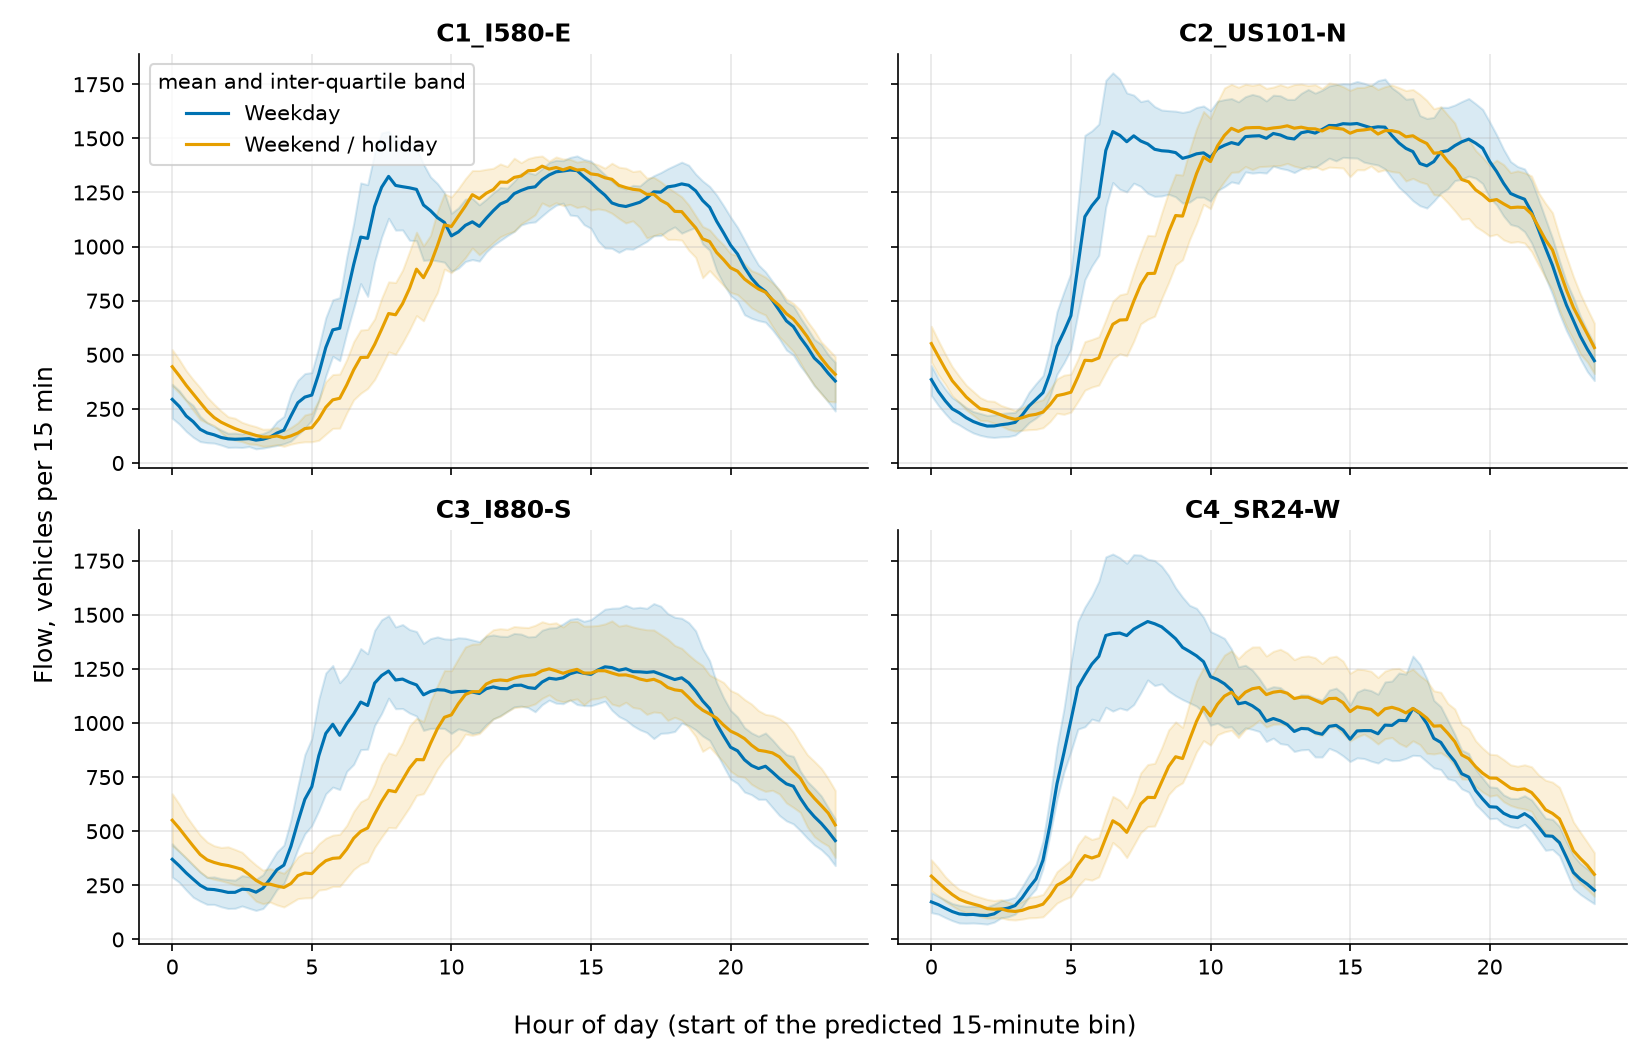
\includegraphics[width=\linewidth]{eda01_daily_profile.png}\caption{Daily profile by corridor and day type.}\end{subfigure}\hfill
\begin{subfigure}{0.48\linewidth}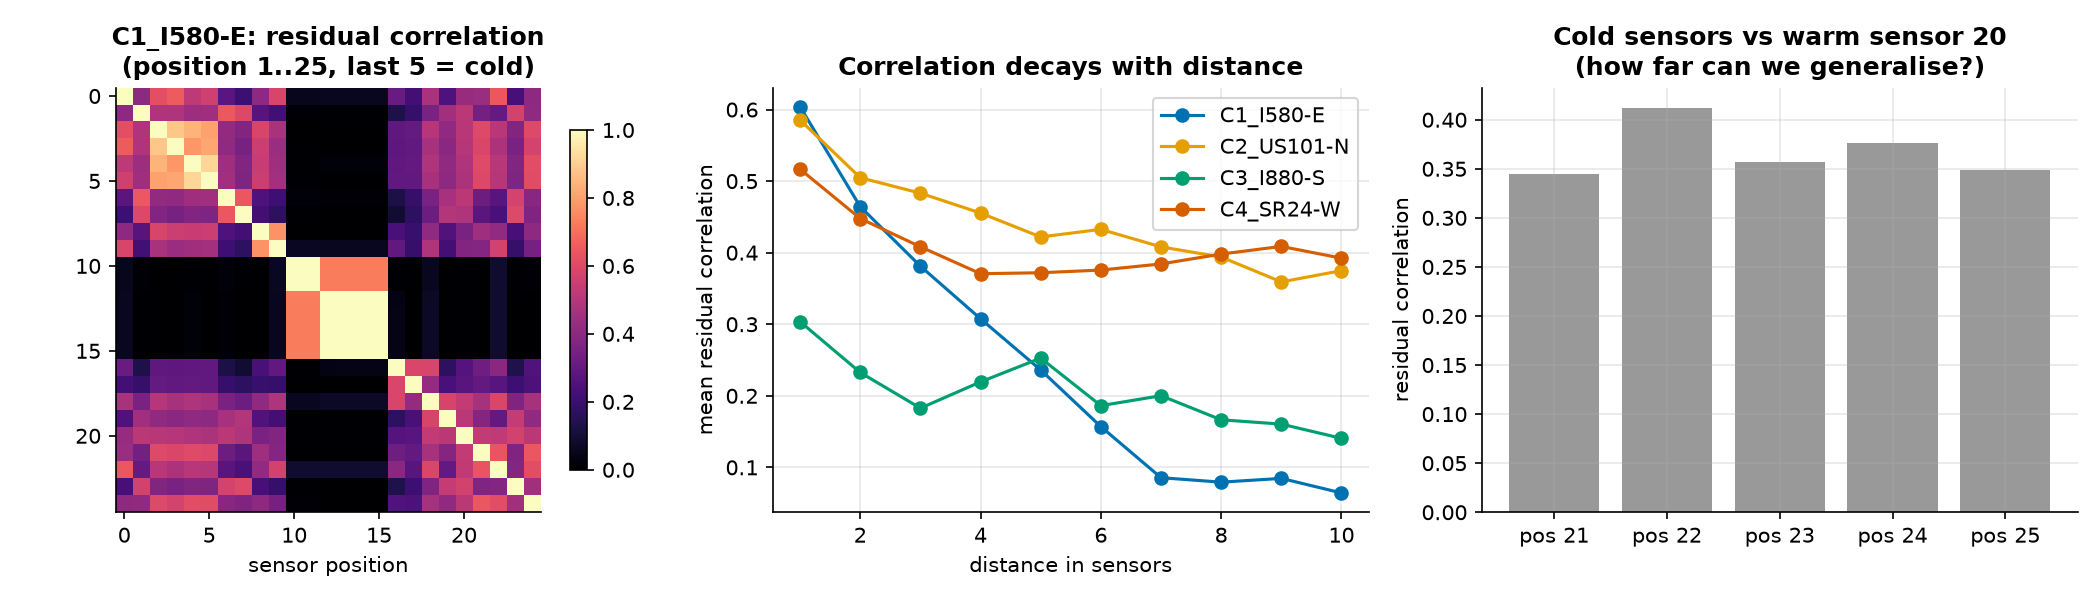
\includegraphics[width=\linewidth]{eda06_spatial_dependence.png}\caption{Correlation of neighbouring sensors.}\end{subfigure}
\caption{Two of the EDA findings.}\label{fig:eda}
\end{figure}

% ---------------------------------------------------------------------------------------------- 4
\section{Preprocessing and feature engineering}\label{sec:prep}
\textbf{Cleaning} (all steps are causal, using only data that ended before the origin).
(i) A 5-minute reading is invalid if it lies in a daytime run of zeros of at least 2 hours, a run of one repeated non-zero value of at
least 2 hours, or exceeds 200 vehicles per lane. (ii) A 15-minute bin is the mean of its three readings times 3 if at least two are valid.
(iii) Remaining gaps are filled with the last value (up to 1 hour), else the same bin one week earlier, else the median of the previous weeks.
Missing \emph{targets} are never imputed; those rows are excluded.\\
\textbf{Scale-free target.} The target is flow divided by the sensor's trailing 7-day mean flow (fallback: 28-day median, at least 5).
Predictions are multiplied back, so all metrics are in vehicles per 15 minutes. This makes busy and quiet sensors comparable.\\
\textbf{Template days and clean rows.} A sensor-day is a template day if at least 90\% of its valid bins equal the same bin 7 days before or
after (rule fixed on 2017--2018). We keep these rows in the main results and also report a \emph{clean rows} view (template days removed; 87.2\% of 2019 rows kept).\\
\textbf{Features.} 31 features in 7 groups (Table~\ref{tab:feat}), computed from the latest completed bin and earlier. Calendar features
describe the target bin, since the calendar of the future is known; weather is taken at the origin. A row is dropped if a feature or the target is missing.

\begin{table}[H]\centering\small
\begin{tabular}{llp{9.6cm}}
\toprule Group & \# & Features \\ \midrule
Lags & 7 & flow now and 15, 30, 45, 60, 120 minutes earlier; share of the last 3 hours missing \\
Rolling & 6 & mean and standard deviation over 1 h and 3 h, 24 h mean, the sensor scale \\
Seasonal & 2 & same time last week; mean of the same time over the last 4 weeks \\
Calendar & 7 & time of day and weekday as sine/cosine, month, California holiday, weekend \\
Weather & 4 & precipitation, temperature, wind, rain in the last 3 h \\
Neighbours & 4 & scaled flow of the sensor behind and ahead; flags saying whether they exist \\
Context & 1 & number of lanes \\ \bottomrule
\end{tabular}
\caption{The 31 features.}\label{tab:feat}
\end{table}

% ---------------------------------------------------------------------------------------------- 5
\section{Leakage prevention}
Leakage means using information that would not be available at forecast time. We guard against it in five ways.
\begin{enumerate}
\item \textbf{Causal pipeline.} Imputation, the sensor scale and all features use data before the origin only; the template rule was fixed before 2019 was touched.
\item \textbf{Scramble-the-future test.} All flow and weather data after a cut time are replaced by random numbers and the feature table is
rebuilt; every feature of every earlier origin must be identical. A positive control scrambles the \emph{past} and confirms the features then change, so the test can fail.
\item \textbf{Live-parity test.} A separate builder (\code{src/live.py}) recomputes the feature row from history alone, as a deployed system would; it must equal the training table row for row. It also refuses requests for the future.
\item \textbf{Tuning on 2017--2018 only.} Settings are chosen on validation; 2019 is read only by the final refit and scoring.
\item \textbf{Frozen test predictions.} The 22 test prediction files (9 models $\times$ 2 horizons, plus 2 extra LightGBM seeds per horizon; baselines are computed directly) are fingerprinted in \code{results/FROZEN.json} and the writer refuses to overwrite them. The best baseline is chosen on validation before test scoring.
\end{enumerate}
Twenty automated tests (leakage, parity, data integrity, unit and app tests) pass.

% ---------------------------------------------------------------------------------------------- 6
\section{Split design}
The split is strictly chronological (Table~\ref{tab:split}). Validation is half a year so that it contains autumn and winter; the test is a full year,
so every season and holiday counts. The last 4 origins (one hour) of train and validation are dropped (\emph{purge}) so that features and targets near a
boundary do not overlap the next period. For speed we use one origin in four per sensor, with a shifted pattern so all times of day occur; neighbouring
origins are almost duplicates. Cold sensors contribute only to the test (174,689 rows).

\begin{table}[H]\centering\small
\begin{tabular}{llrrr}
\toprule Split & Period & Rows (15 min) & Warm rows & Cold rows \\ \midrule
Train & 2017-01-29 to 2018-06-30 & 992,997 & 992,997 & 0 \\
Validation & 2018-07-01 to 2018-12-31 & 350,587 & 350,587 & 0 \\
Test & 2019-01-01 to 2019-12-31 & 868,158 & 693,469 & 174,689 \\ \bottomrule
\end{tabular}
\caption{Chronological split.}\label{tab:split}
\end{table}

% ---------------------------------------------------------------------------------------------- 7
\section{Model configurations and tuning}
\textbf{Baselines:} persistence (latest reading), same time last week, and the 4-week average of the same time. On validation the best is
persistence at 15 minutes and the 4-week average at 60 minutes. \textbf{Models} (all on the same 31 features and the scaled target):
Ridge; PCA then Ridge; a Decision Tree; a Random Forest (150 trees, 30\% row samples);
AdaBoost; Gradient Boosting; XGBoost; LightGBM; CatBoost, using scikit-learn where applicable. All are trained with squared-error loss (L2; AdaBoost uses its linear loss) and ranked and early-stopped on MAE.

\textbf{Protocol} (identical for every model and horizon). (1) \emph{Tune} on a 300,000-row month-stratified subset of the training rows,
scoring each candidate on the full validation split by MAE; large spaces use random search (4 to 8 draws), small ones a full grid; the boosters stop early
(patience 100) on validation MAE. (2) \emph{Fit} the best setting on all training rows. (3) \emph{Refit} on train plus validation with the tree count fixed,
and predict 2019 once. (4) \emph{Freeze} the predictions. Our first AdaBoost grid (shallow trees, large rates) sat on the grid edge and lost to the baselines, so we widened it to deeper trees and smaller rates.
A wider search for LightGBM, XGBoost and CatBoost lowered validation MAE by only 0.3--1.2\%, so the ranking is stable.

\begin{table}[H]\centering\small
\begin{tabular}{llp{5.7cm}r}
\toprule Model & Horizon & Selected settings & Trees \\ \midrule
Ridge / PCA+Ridge & both & $\alpha=0.01$; PCA keeps all 31 components & -- \\
Decision Tree & 15 / 60 & depth 14, min leaf 100 / 50 & -- \\
Random Forest & 15 / 60 & min leaf 20, max features 0.5 / 0.33 & 150 \\
AdaBoost & both & base depth 12, learning rate 0.02 & 100 \\
Gradient Boosting & both & depth 5, learning rate 0.1 & 300 \\
XGBoost & both & depth 8, learning rate 0.05, no subsampling & 1943 / 2088 \\
LightGBM & both & 127 leaves, min child 300, $\lambda=10$, rate 0.05 & 1414 / 1695 \\
CatBoost & 15 / 60 & depth 8, rate 0.1, L2 leaf reg.\ 3 / 10 & 2000 (cap) \\ \bottomrule
\end{tabular}
\caption{Selected hyperparameters (chosen on validation).}\label{tab:set}
\end{table}

% ---------------------------------------------------------------------------------------------- 8
\section{Evaluation results}
Metrics: MAE (headline), RMSE, WAPE (total absolute error over total flow) and \emph{skill} $=1-\mathrm{MAE}/\mathrm{MAE}_{\text{best baseline}}$ (the best baseline is chosen on validation).
Intervals are 95\% day-block bootstrap intervals (whole days are resampled, since rows within a day are correlated).

\begin{table}[H]\centering\small
\begin{tabular}{lrrrrrr}
\toprule & \multicolumn{3}{c}{15 minutes} & \multicolumn{3}{c}{60 minutes} \\
\cmidrule(lr){2-4}\cmidrule(lr){5-7}
Model & MAE & 95\% interval & Skill & MAE & 95\% interval & Skill \\ \midrule
Persistence & 66.38 & 65.57--67.12 & 0.0\% & 142.01 & 140.45--143.46 & -81.1\% \\
Last week & 91.78 & 88.45--95.43 & -38.3\% & 91.74 & 88.44--95.42 & -17.0\% \\
4-week average & 78.44 & 75.65--81.43 & -18.2\% & 78.43 & 75.61--81.43 & 0.0\% \\ \midrule
Ridge & 55.98 & 55.32--56.69 & +15.7\% & 75.26 & 73.83--76.72 & +4.0\% \\
PCA + Ridge & 55.98 & 55.32--56.69 & +15.7\% & 75.26 & 73.83--76.72 & +4.0\% \\
Decision Tree & 52.50 & 51.88--53.12 & +20.9\% & 67.12 & 66.06--68.16 & +14.4\% \\
Random Forest & 49.55 & 48.94--50.19 & +25.3\% & 62.35 & 61.36--63.29 & +20.5\% \\
AdaBoost & 51.12 & 50.52--51.76 & +23.0\% & 65.81 & 64.76--66.80 & +16.1\% \\
Gradient Boosting & 50.78 & 50.17--51.42 & +23.5\% & 64.31 & 63.34--65.25 & +18.0\% \\
XGBoost & 48.73 & 48.08--49.39 & +26.6\% & 61.29 & 60.40--62.18 & +21.9\% \\
\textbf{LightGBM} & \textbf{48.63} & 47.98--49.28 & \textbf{+26.7\%} & \textbf{61.15} & 60.27--62.02 & \textbf{+22.0\%} \\
CatBoost & 48.96 & 48.33--49.61 & +26.2\% & 61.58 & 60.67--62.49 & +21.5\% \\ \bottomrule
\end{tabular}
\caption{Test results on 2019 (all 868,158 rows). MAE in vehicles per 15 minutes; skill is against the best baseline for that horizon.}\label{tab:res}
\end{table}

\textbf{Reading.} There are three tiers: baselines, the linear model, and the tree models, which all gain more at 60 minutes. LightGBM also has the best RMSE (77.50 / 97.57) and WAPE (5.31\% / 6.67\%).
A paired day-block bootstrap shows LightGBM beats every other model in 100\% of resamples, but only by 0.11 vehicles over XGBoost (interval 0.06--0.15) and 0.33 over CatBoost at 15 minutes (0.14 and 0.42 at 60), so the top three are practically tied; Random Forest trails by 0.92 (1.20), Gradient Boosting by 2.15 (3.15).
Validation MAE for LightGBM (47.97 / 62.00) is close to its test MAE, so the tuned model transfers to a new year, and three random seeds give test MAEs that differ by only 0.02 (mean 48.62 / 61.17, standard deviation 0.019 / 0.016), so the result does not depend on a lucky seed.
The lead is not an artefact of the annual average: LightGBM has the lowest MAE in each quarter of 2019 at both horizons (by a small margin over XGBoost and CatBoost) and beats the best baseline in every quarter, by 24.9--27.8\% at 15 minutes and 18.7--25.5\% at 60 minutes.
\textbf{PCA + Ridge equals Ridge} because validation chose all 31 components, and a full rotation keeps all information (Section~\ref{sec:pca}).

\subsection{Warm and cold sensors, and clean rows}\label{sec:clean}
Cold sensors are only about 0.6 WAPE points worse than warm ones for every model (LightGBM: 5.19\% vs 5.80\% at 15 minutes, 6.55\% vs 7.19\% at 60). On the clean rows (template days removed) LightGBM reaches MAE 54.2 and 67.2, so the all-rows headline is flattering; the 8 template sensors are nearly free to predict. We report both.

\subsection{PCA study}\label{sec:pca}
Beyond PCA+Ridge we refit Ridge, Decision Tree, Random Forest and LightGBM on the first $k$ principal components (validation only). 14 components explain 90\% of the variance and 22 explain 99\%, but every cut raises the error: e.g.\ LightGBM at 15 minutes goes from 50.3 (no PCA, on the study's smaller training subset, so not comparable to the 47.97 above) to 81.6, 70.0, 64.0 and 54.7 for $k=4, 8, 15, 31$ respectively. Ridge returns to its original error only at $k=31$; trees get worse even at $k=31$, since rotation mixes the meaningful features. PCA therefore does not help here and we keep the 31 original features.

\subsection{Cost and comparison with published results}
\textbf{Cost.} Fit times (15 / 60 min): Ridge 5 s, Decision Tree 44 / 65 s, XGBoost 189 / 203 s, LightGBM 147 / 233 s, CatBoost 640 / 388 s, Random Forest 273 / 159 s (a 290 MB model), Gradient Boosting 2480 / 2107 s and AdaBoost 7250 / 3799 s. LightGBM gives the best accuracy at a small size (about 20 MB) and fits in under four minutes, so the best model is also cheap enough to retrain often.

\textbf{Published results.} The LargeST benchmark \cite{largest} reports LSTM, DCRNN, Graph WaveNet \cite{gwnet} and D2STGNN \cite{d2stgnn} on all Bay Area sensors, at 45 and 90 minutes, with its own split, so absolute errors are not comparable and we do not put them in one table. The fair way to compare is relative to a naive forecast on the same data. Table~\ref{tab:pub} does this with the MAE ratio to persistence (lower is better).
\begin{table}[H]\centering\small
\begin{tabular}{lcr}
\toprule Method & Horizon & MAE / persistence MAE \\ \midrule
\textbf{Ours: LightGBM (100 sensors, 2019 test)} & \textbf{15 min} & \textbf{0.73} \\
LSTM / DCRNN / Graph WaveNet / D2STGNN (LargeST) & 45 min & 0.63 / 0.57 / 0.55 / 0.54 \\
\textbf{Ours: LightGBM} & \textbf{60 min} & \textbf{0.43} \\
LSTM / DCRNN / Graph WaveNet / D2STGNN (LargeST) & 90 min & 0.51 / 0.43 / 0.39 / 0.39 \\ \bottomrule
\end{tabular}
\caption{Error relative to persistence. The horizons differ, so rows are read as ``how much of the naive error is left'', not as a ranking.}\label{tab:pub}
\end{table}
We read this as follows. (1) Our relative error at 60 minutes (0.43) is in the same range as the published deep graph models at 90 minutes (0.39--0.51; DCRNN's is 0.43) and below their LSTM's 0.51, although persistence is a harder target to beat at a long horizon, so the comparison is only indicative. (2) The published models are trained on several thousand sensors with a learned road graph, whereas ours uses 100 sensors, hand-built features and one tree model per horizon, fitted in minutes and explained feature by feature with TreeSHAP. (3) The result is held to a stricter standard: a calendar-year test that was scored once, frozen predictions, a scramble-the-future leakage test, a live-parity test, tuning on validation only, day-block bootstrap intervals, a paired bootstrap between models, and 20 automated tests. (4) We test generalisation to 20 sensors never seen in training, which cost only 0.6 WAPE points, and we report where the model fails (outages, sudden changes, holidays). (5) The whole pipeline, from raw data to a working app, is reproducible from the repository. We still make no claim to beat the graph models: the setups differ, and a graph model is the natural next step.

% ---------------------------------------------------------------------------------------------- 9
\Needspace{8\baselineskip}
\section{Additional analyses}
We completed all six analyses of the brief. The three main ones, \textbf{A (feature-group ablation), D (robustness) and E (error analysis)}, are done in detail (Sections 9.1 to 9.3). The other three, \textbf{B (error patterns), C (efficiency) and F (feature importance)}, were quick checks: we tried them and report what we observed (Section 9.4).
\subsection{Analysis A: feature-group ablation}
For each model and horizon we refit with frozen settings on a training subset, dropping one feature group at a time, and score on validation. Table~\ref{tab:abl} gives the percentage increase in MAE when a group is removed.
At 15 minutes the \textbf{lags} matter most, with the calendar nearly as important for boosted trees; at 60 minutes the \textbf{seasonal} and \textbf{calendar} groups dominate. \textbf{Weather and neighbours add nothing measurable} (weather is slightly negative for the boosters). Ridge depends heavily on the weekly value at 60 minutes (+29.6\%), since a linear model has no other way to know the weekly pattern.
Permutation importance agrees: for LightGBM at 15 minutes the latest flow alone carries about 96\% of the split gain. Feature selection by group is what this ablation measures; the effect of dimensionality reduction (PCA) is analysed separately in Section~\ref{sec:pca}, where it never helped.

\begin{table}[H]\centering\small
\begin{tabular}{llrrrrrrr}
\toprule Horizon & Model & Lags & Rolling & Seasonal & Calendar & Weather & Neighb. & Context \\ \midrule
15 min & Ridge & +13.4 & +0.5 & +4.4 & +1.3 & -0.0 & -0.1 & +0.0 \\
 & Random Forest & +10.3 & +1.0 & +3.4 & +1.6 & -0.1 & -0.3 & -0.0 \\
 & LightGBM & +5.0 & +1.1 & +2.0 & +4.8 & -0.5 & -0.0 & +0.1 \\ \midrule
60 min & Ridge & +4.2 & +0.9 & +29.6 & +1.8 & -0.1 & +0.3 & +0.0 \\
 & Random Forest & +3.7 & +1.8 & +9.1 & +4.2 & -0.3 & -0.8 & -0.2 \\
 & LightGBM & +2.0 & +2.4 & +6.6 & +8.1 & -1.0 & +0.2 & +0.4 \\ \bottomrule
\end{tabular}
\caption{Increase in validation MAE (\%) when one feature group is removed (three representative models; all nine models at 15 minutes are in Figure~\ref{fig:abl}, and all results are in \code{results/ablation/}).}\label{tab:abl}
\end{table}

\begin{figure}[H]\centering
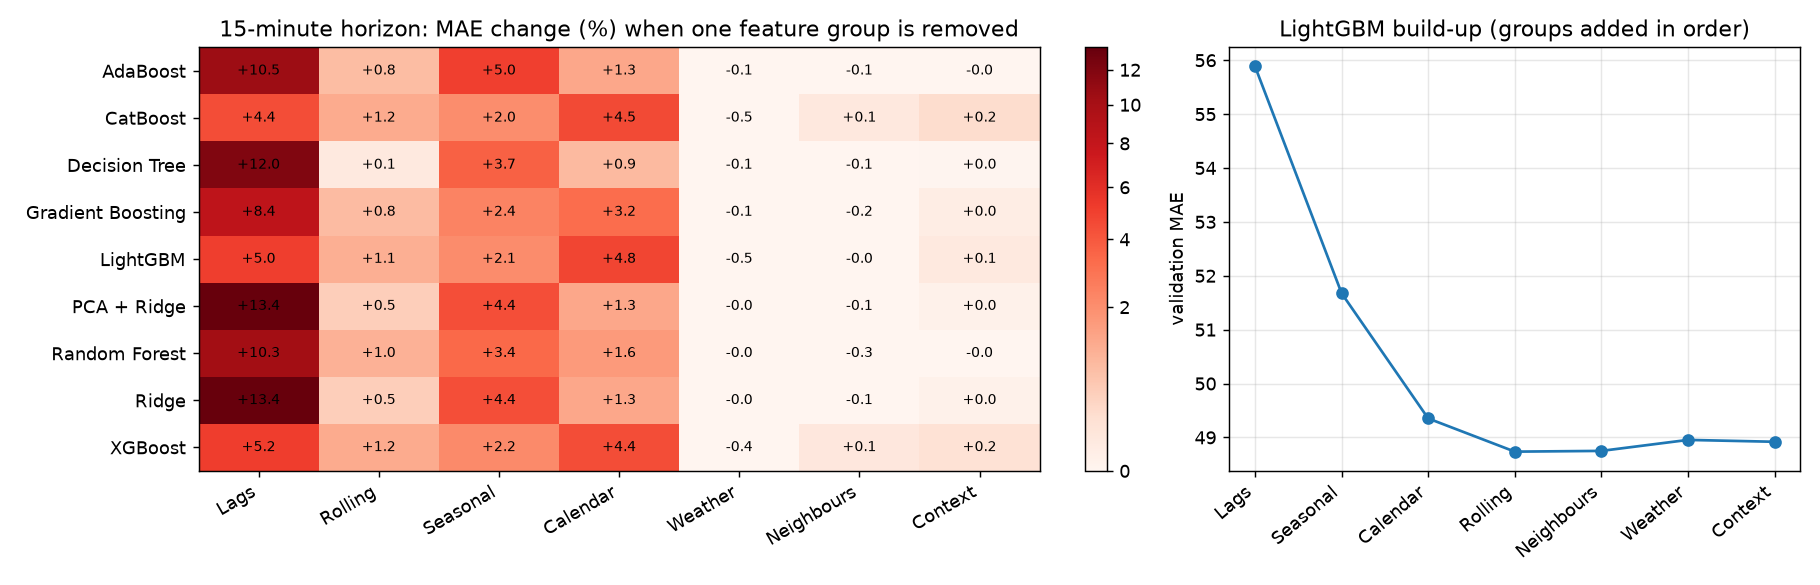
\includegraphics[width=\linewidth]{ablation_h15.png}
\caption{Feature-group ablation for all nine models at 15 minutes.}\label{fig:abl}
\end{figure}

\subsection{Analysis D: robustness and sensitivity}
Models are fitted once with frozen settings and stressed on validation: multiplicative noise on the five lag readings; the latest reading missing (replaced by the one before, as a live system would); only the last $m$ months of training data; and refitting on half the warm sensors and scoring on the other half. Table~\ref{tab:rob} gives the MAE increase.
\textbf{Noise hurts far more than missing data} (a wrong reading misleads the model, a missing one is replaced by a nearly as good value), and the 15-minute model is more fragile because it leans on the latest values. Boosted trees need history (only 3 months costs LightGBM +8.7\% and +13.3\%), whereas Ridge barely cares. Unseen sensors cost little at 15 minutes and more at 60. The noise test touches only the lags, so it understates the harm of a truly noisy sensor. The 3-month history test was run for three models (Ridge, Decision Tree, LightGBM); the other tests cover all nine (Table~\ref{tab:rob}, Figure~\ref{fig:rob}).
\textbf{Implications for deployment.} A live system should put its effort into detecting and filtering bad or noisy sensor readings, since a gap can be filled almost for free but a wrong value cannot; boosted trees should be trained on at least a year of history (12 months costs under 1\%, 6 months about 7\%); and a newly installed sensor can be forecast 15 minutes ahead at a small cost (+3.3\% for LightGBM) but needs its own history before 60-minute forecasts are trusted (+8.1\%).

\begin{table}[H]\centering\small
\begin{tabular}{lrrrrrrrr}
\toprule & \multicolumn{4}{c}{15 minutes} & \multicolumn{4}{c}{60 minutes} \\
\cmidrule(lr){2-5}\cmidrule(lr){6-9}
Model & Noise & Miss. & Unseen & 3 mo & Noise & Miss. & Unseen & 3 mo \\ \midrule
Ridge & +28.0 & +6.5 & +0.1 & +1.7 & +8.8 & +2.2 & +0.7 & +0.5 \\
PCA + Ridge & +27.8 & +6.4 & +0.1 & -- & +8.8 & +2.1 & +0.7 & -- \\
Decision Tree & +28.3 & +6.8 & +2.6 & +8.1 & +8.4 & +1.9 & +3.5 & +11.9 \\
Random Forest & +23.2 & +6.7 & +2.0 & -- & +6.3 & +1.7 & +3.8 & -- \\
AdaBoost & +27.4 & +6.6 & +1.5 & -- & +5.9 & +1.3 & +2.0 & -- \\
Gradient Boosting & +22.7 & +6.0 & +1.3 & -- & +5.7 & +1.4 & +3.1 & -- \\
XGBoost & +29.0 & +6.4 & +4.4 & -- & +10.3 & +1.9 & +8.7 & -- \\
LightGBM & +26.0 & +6.3 & +3.3 & +8.7 & +8.8 & +2.0 & +8.1 & +13.3 \\
CatBoost & +26.9 & +6.5 & +3.1 & -- & +8.6 & +2.0 & +6.7 & -- \\ \bottomrule
\end{tabular}
\caption{Increase in validation MAE (\%) under stress: noise = 10\% multiplicative noise on the lag readings; Miss.\ = latest reading missing in 30\% of rows; Unseen = scored on sensors not used in training; 3 mo = only 3 months of training history (``--'' = not run).}\label{tab:rob}
\end{table}

\begin{figure}[H]\centering
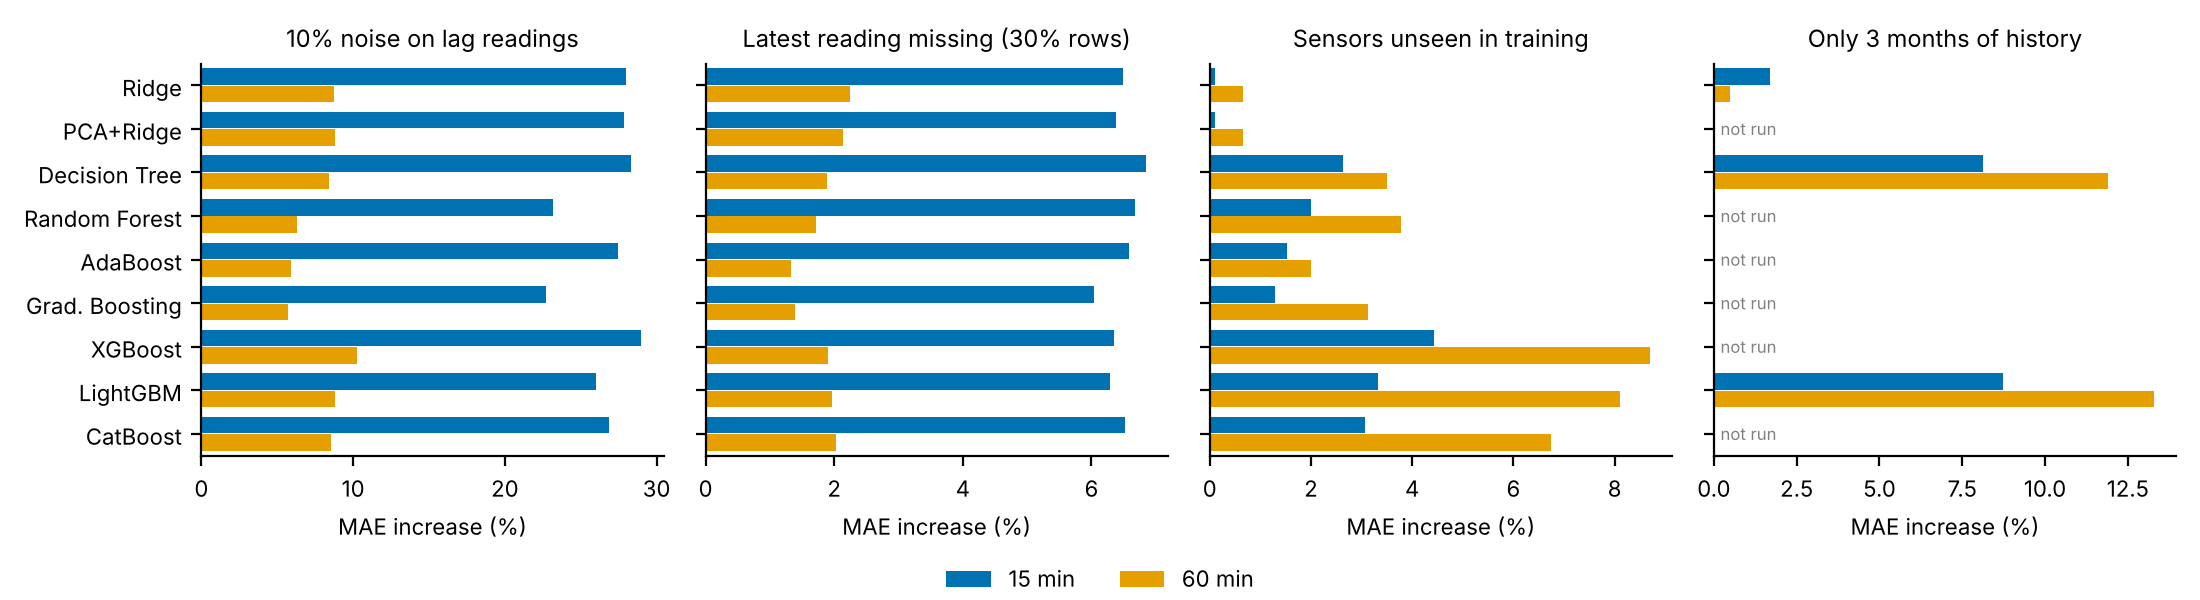
\includegraphics[width=\linewidth]{robust_summary.png}
\caption{Robustness of all nine models (validation MAE increase, \%; blue 15 minutes, orange 60 minutes).}\label{fig:rob}
\end{figure}

\subsection{Analysis E: error analysis}
We split the 2019 errors of the final model by segment (WAPE, \%; Table~\ref{tab:err}). The hard cases are \textbf{sudden changes} (WAPE roughly triples from the steadiest to the most sudden quartile), \textbf{holidays}, \textbf{rain} and \textbf{low flow} (a small count gives a larger percentage). Peak hours are not especially hard.
The worst 1\% of rows carry about 8\% of the total absolute error and are mostly \textbf{feed outages}: on 2019-09-20 at 12:00, 18 of the 100 sensors read exactly 0 and 30 were below 20\% of their usual level. No feature can predict a dropout, so part of the error is data quality, not forecasting.
\textbf{Across models} (Figure~\ref{fig:err}) all nine models struggle in the same places, so these are properties of the data, not of one method. The differences lie in how badly: Ridge degrades much more than the boosted trees on holidays (WAPE 1.35$\times$ LightGBM's at 15 minutes and 1.71$\times$ at 60), at low flow (1.27$\times$, 1.38$\times$) and on sudden changes (1.23$\times$, 1.30$\times$), while XGBoost, CatBoost and LightGBM stay within about 0.3 WAPE points of each other in every segment. The Random Forest is slightly better than LightGBM on the steadiest 15-minute rows (2.91\% vs 3.06\%), and every model is worst on the same segments.

\begin{table}[H]\centering\small
\begin{tabular}{llrr}
\toprule Segment & Level & 15 min & 60 min \\ \midrule
Time of day & off-peak / peak & 5.43 / 5.04 & 6.85 / 6.29 \\
Day type & weekday / weekend / holiday & 5.35 / 5.11 / 6.04 & 6.69 / 6.39 / 8.62 \\
Weather & dry / rain & 5.25 / 5.87 & 6.58 / 7.61 \\
Change since last reading & steadiest / most sudden quartile & 3.06 / 9.55 & 4.52 / 10.36 \\
Flow level & low / mid / high & 8.18 / 5.73 / 4.24 & 11.17 / 7.09 / 5.19 \\
Sensor role & warm / cold & 5.19 / 5.80 & 6.55 / 7.19 \\ \bottomrule
\end{tabular}
\caption{LightGBM WAPE (\%) by segment on the 2019 test year.}\label{tab:err}
\end{table}

\begin{figure}[H]\centering
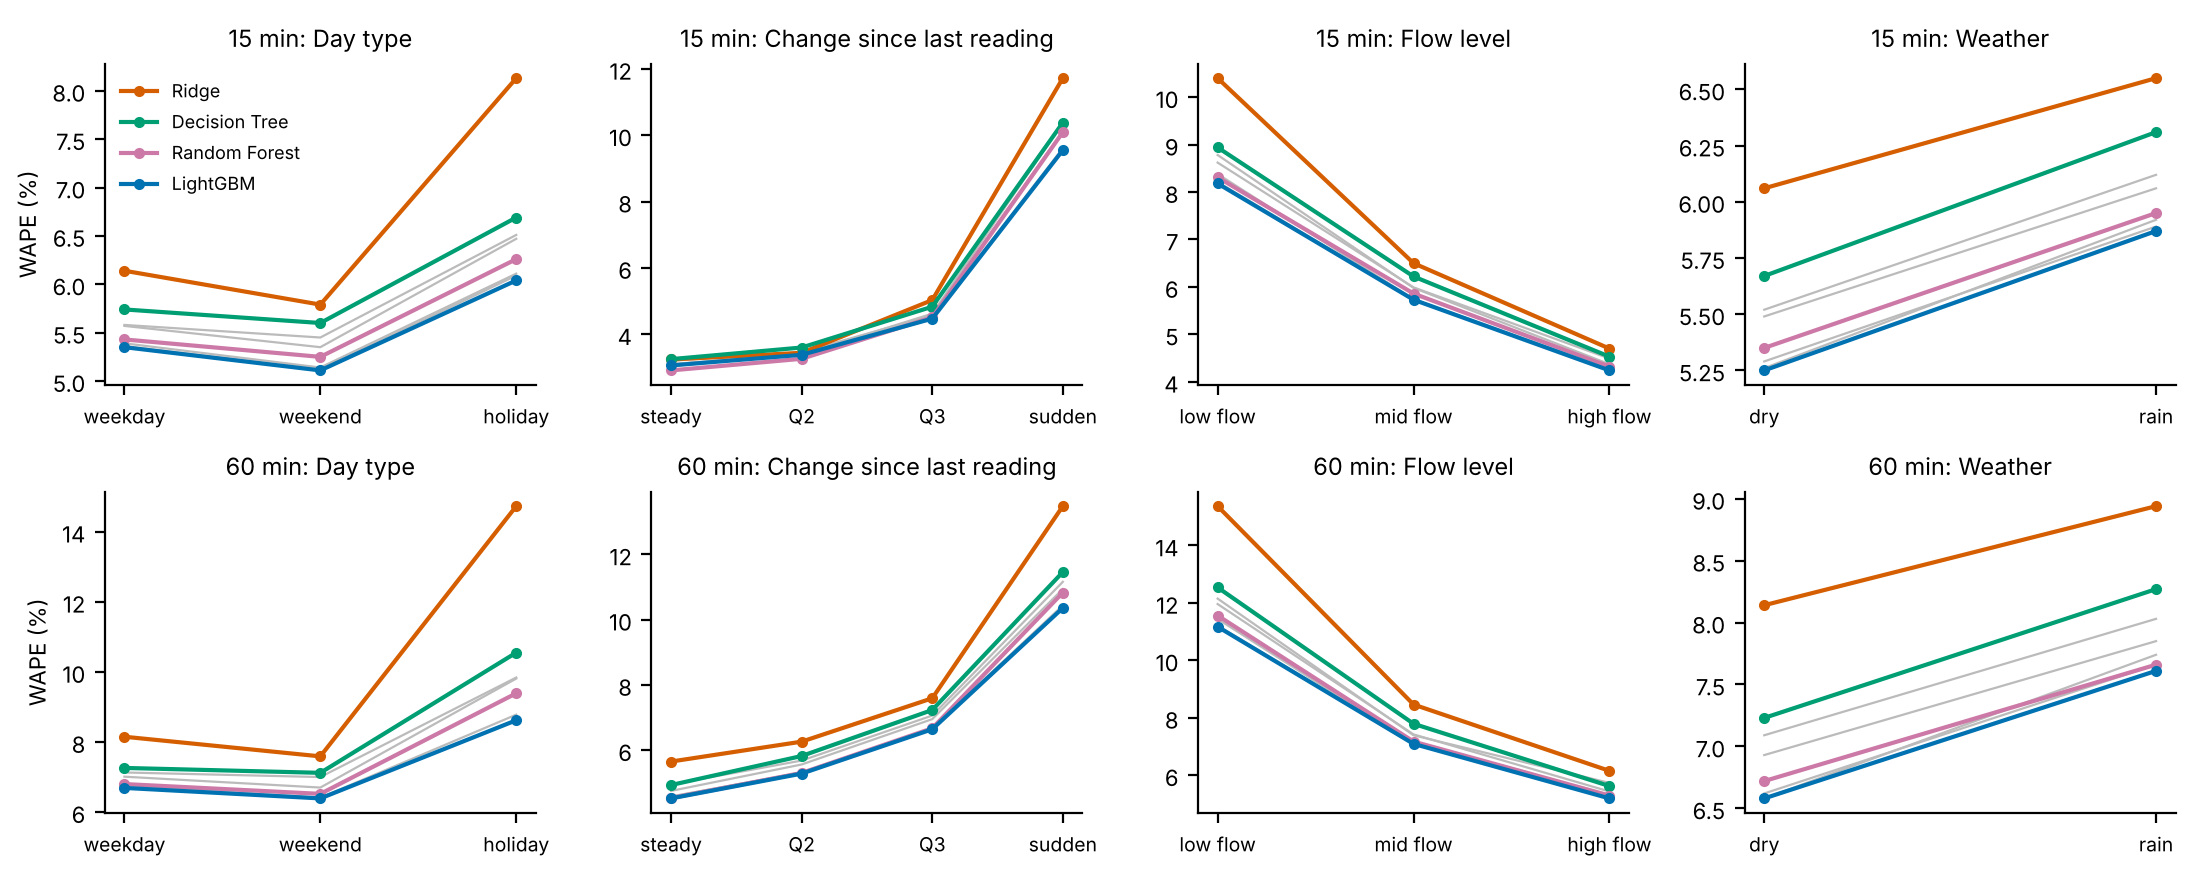
\includegraphics[width=\linewidth]{err_models_segments.png}
\caption{Test-year WAPE (\%) by segment for Ridge, Decision Tree, Random Forest and LightGBM (grey: the other boosters and PCA + Ridge).}\label{fig:err}
\end{figure}

\subsection{Analyses B, C and F: tried and observed}
\textbf{B, error patterns:} WAPE by quarter and corridor (2019, LightGBM) shows the error is highest in the first quarter (5.9\% at 15 minutes, falling to 5.0\% in the last) and on the I-880 and SR-24 corridors (5.8--5.9\%, against 4.9\% on I-580 and US-101); the per-sensor spread is wide (1.0\% to 11.3\%), with the template sensors lowest.
\textbf{C, efficiency:} XGBoost and LightGBM reach the best accuracy in 2--4 minutes of fitting and 17--32 MB, while AdaBoost (up to 2 hours) and Random Forest (290 MB) cost most for less accuracy.
\textbf{F, importance:} permutation importance and gain agree; at 15 minutes the latest flow dominates (shuffling it adds 316 vehicles to MAE, about 96\% of gain), at 60 minutes the 4-week same-time average does (about 93\%), so the models use persistence for the short term and the weekly pattern for the long term.
Two validation-only checks, the PCA study (Section 8.2) and a tuning-sensitivity study (Section 7), left the frozen models unchanged.

% ---------------------------------------------------------------------------------------------- 10
\section{User interface}
The app is a Streamlit page (\code{streamlit run app/streamlit\_app.py}) that runs offline on a laptop; the 15-minute data table, the sensor and weather files and the two final LightGBM models are committed in the repository, so it works after a plain clone.
The user picks a horizon, a corridor, a sensor and a date and time (or one of four quick examples). The app rebuilds the features from the history before that time only (the same code as the live-parity test) and shows the \textbf{forecast}, an \textbf{80\% interval} (from the 10th and 90th percentiles of validation errors, an empirical band rather than a guarantee), the latest reading and, if the time has passed, the actual flow and the model error.
Five tabs: \emph{Forecast} (last 24 hours, the same hours a week earlier, the forecast with its interval, and the three baselines); \emph{Corridor view} (all 25 sensors of the corridor); \emph{Why this forecast} (the ten features that moved this prediction most, by TreeSHAP, and per group); \emph{Model performance} (the benchmark tables and figures); \emph{About}.
A \emph{stress test} marks the latest reading missing or adds 0--30\% noise (analysis D made interactive). The app warns when the chosen time lies in the training years, shows a clear message when a data file is missing, and is covered by five automated interaction tests.

\begin{figure}[H]\centering
\begin{subfigure}{0.34\linewidth}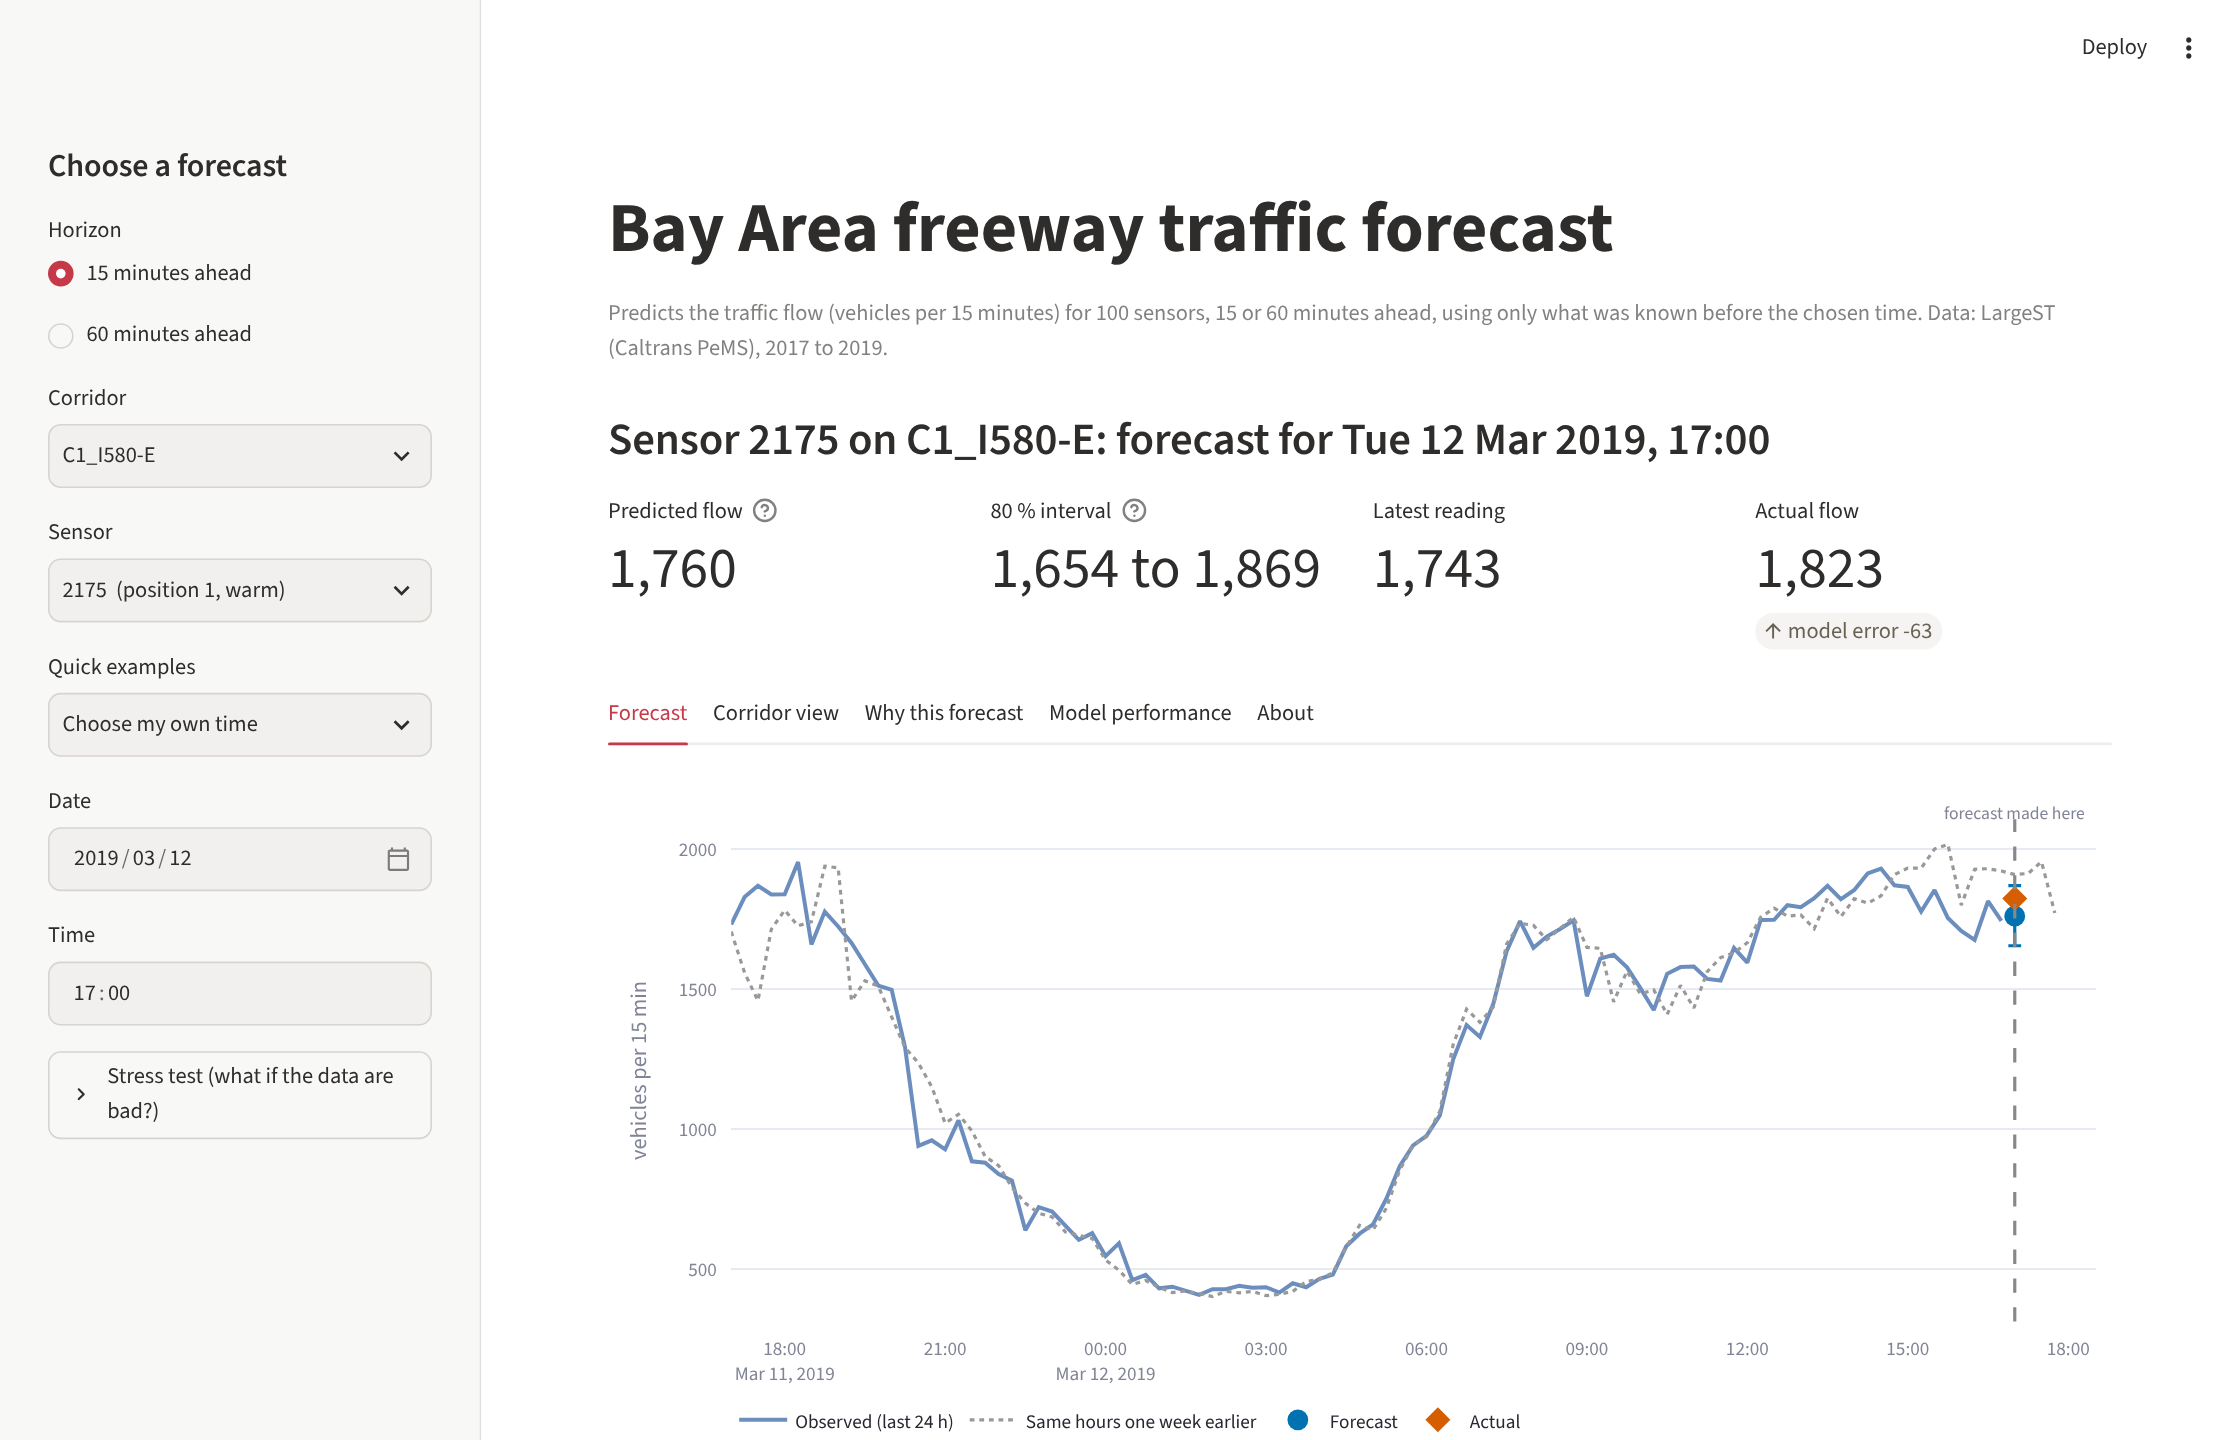
\includegraphics[width=\linewidth]{app_forecast.png}\caption{Forecast tab.}\end{subfigure}\hfill
\begin{subfigure}{0.34\linewidth}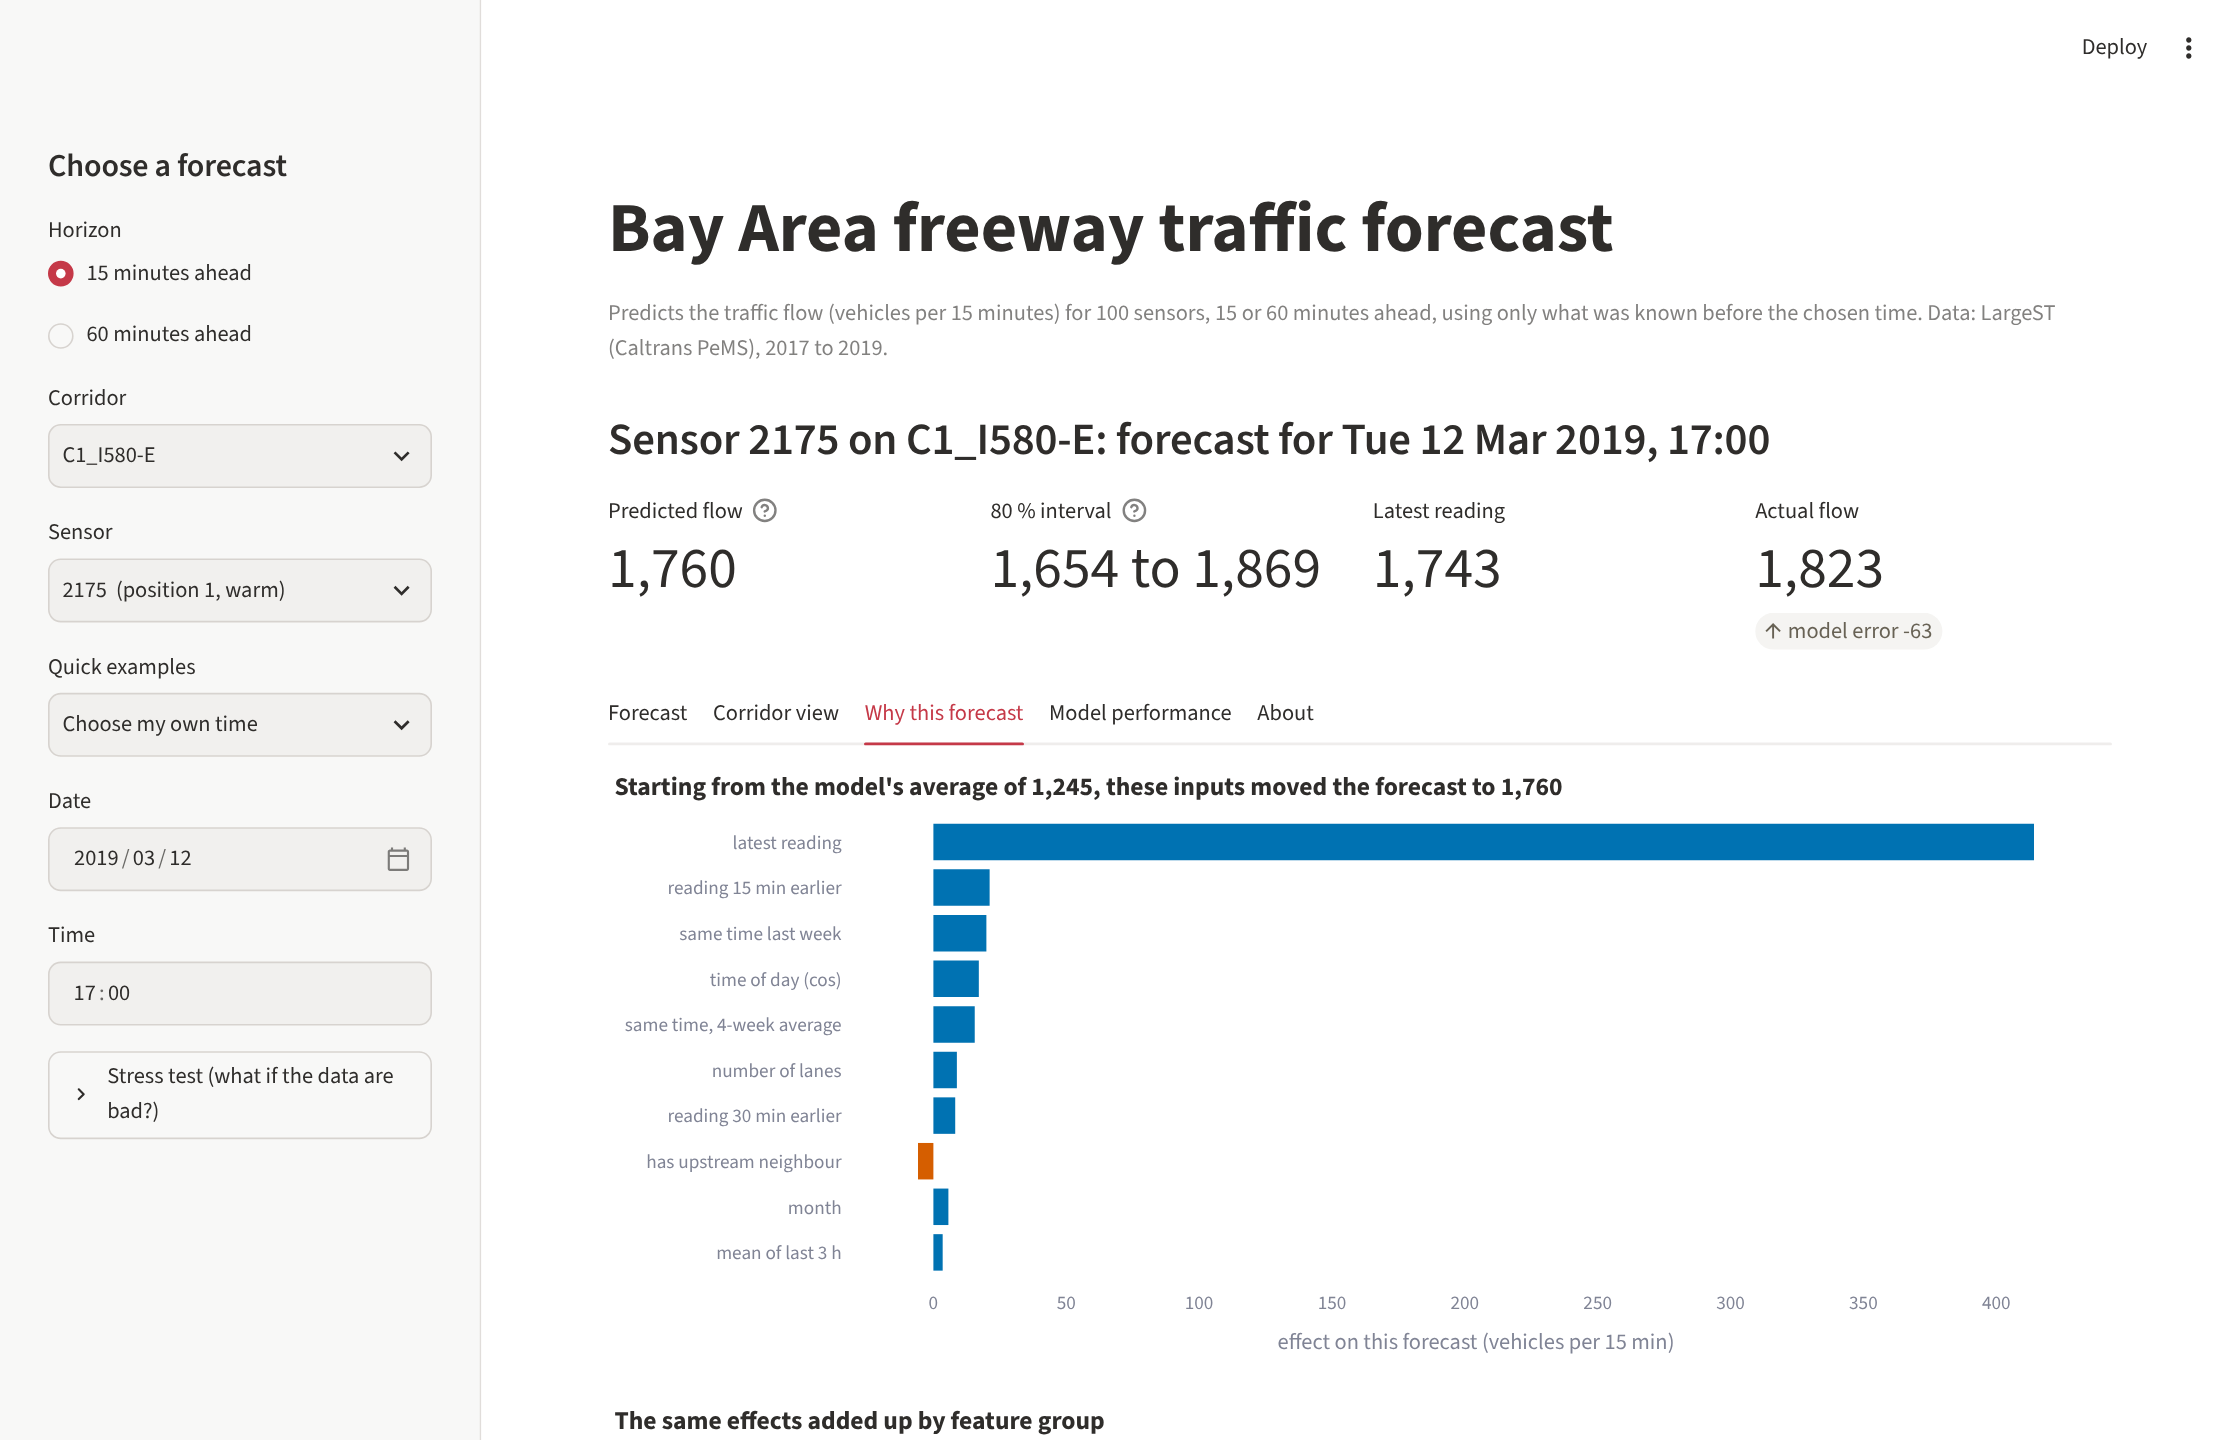
\includegraphics[width=\linewidth]{app_explain.png}\caption{Explanation tab.}\end{subfigure}
\caption{The Streamlit app.}
\end{figure}

% ---------------------------------------------------------------------------------------------- 11
\section{Limitations and conclusions}
\textbf{Limitations.} (1) The headline is flattered by template sensor-days (about 10\%), so the clean-rows view is the fairer one. (2) Feed outages cause the largest errors and cannot be forecast. (3) Weather is reanalysis taken at the origin, not a forecast, and added nothing. (4) The tuning budget is small and the top three models are practically tied. (5) The data is 100 sensors on four corridors in one region, up to 2019, and we tried no graph model. (6) The app's interval is an empirical band, and the model cannot see incidents that the recent readings do not show.

\textbf{Conclusions.} We built and tested a complete traffic forecasting pipeline: 100 Bay Area sensors, 15-minute data cleaned without using the future, 31 features in seven groups, and nine models, with three simple baselines as the reference, tuned on validation and scored once on the unseen year 2019.
The main finding is that gradient-boosted trees, led by LightGBM, cut the error of the best baseline by 26.7\% at 15 minutes (MAE 48.63 against 66.38) and 22.0\% at 60 minutes (61.15 against 78.43), and the gain holds in every quarter of 2019 and across random seeds, while sensors never seen in training are only 0.6 WAPE points worse. XGBoost and CatBoost are statistically indistinguishable in practice, so the choice among the three can follow cost and convenience; LightGBM is the best on accuracy, size and speed together.

The analyses explain why. Recent flow carries the 15-minute forecast and last week's pattern with the calendar carries the 60-minute one; weather and neighbour readings add nothing measurable, and PCA never helps. The models cope with a missing latest reading far better than with a noisy one, and they need about a year of history. The largest errors come from data outages, sudden changes and holidays, which are limits of the data rather than of one method.

Leakage controls make these numbers trustworthy: a chronological split with a purge, tuning on validation only, a scramble test with a positive control, a live-parity test and frozen test predictions. Compared with published graph networks, our error relative to persistence at 60 minutes is in the same range as theirs at 90 minutes, with a model that is far smaller, faster to train and explainable, which we regard as a strong result for this scale; we do not claim to beat them.
The result is also usable: the Streamlit app gives a forecast, an 80\% interval and a per-prediction explanation from the same code as the tests. Next steps are a measured weather and incident feed, a graph model for the neighbour structure, and a wider tuning search.

\begin{thebibliography}{9}\footnotesize\setlength{\itemsep}{0pt}
\bibitem{largest} LargeST benchmark dataset (Bay Area traffic, 2017--2019; also the source of the published comparison results). X.~Liu et al., NeurIPS Datasets and Benchmarks 2023. \url{https://github.com/liuxu77/LargeST}
\bibitem{pems} Caltrans Performance Measurement System (PeMS), the original loop-detector data. \url{https://pems.dot.ca.gov}
\bibitem{openmeteo} Open-Meteo historical weather API (ERA5 reanalysis), hourly precipitation, temperature and wind. \url{https://open-meteo.com}
\bibitem{gwnet} Z.~Wu et al. Graph WaveNet for deep spatial-temporal graph modeling. IJCAI 2019 (comparison method). \url{https://arxiv.org/abs/1906.00121}
\bibitem{d2stgnn} Z.~Shao et al. Decoupled dynamic spatial-temporal graph neural network for traffic forecasting. PVLDB 2022 (comparison method). \url{https://arxiv.org/abs/2206.09112}
\end{thebibliography}
\end{document}
